\begin{frame}
	\frametitle{SeismoCloud: come funziona}
	
	\begin{enumerate}
		\item<1-> Tanti sismometri installati dagli utenti (dispositivi IoT e/o App per cellulari)
		\item<2-> I sismometri analizzano le vibrazioni, e segnalano al server quelle "interessanti"
		\item<3-> Il server mette in relazione le segnalazioni
		\item<4-> Se i dati mostrano un terremoto, il server notifica la app su smartphones
	\end{enumerate}
	
\end{frame}
\begin{frame}
	\frametitle{SeismoCloud: come funziona}

	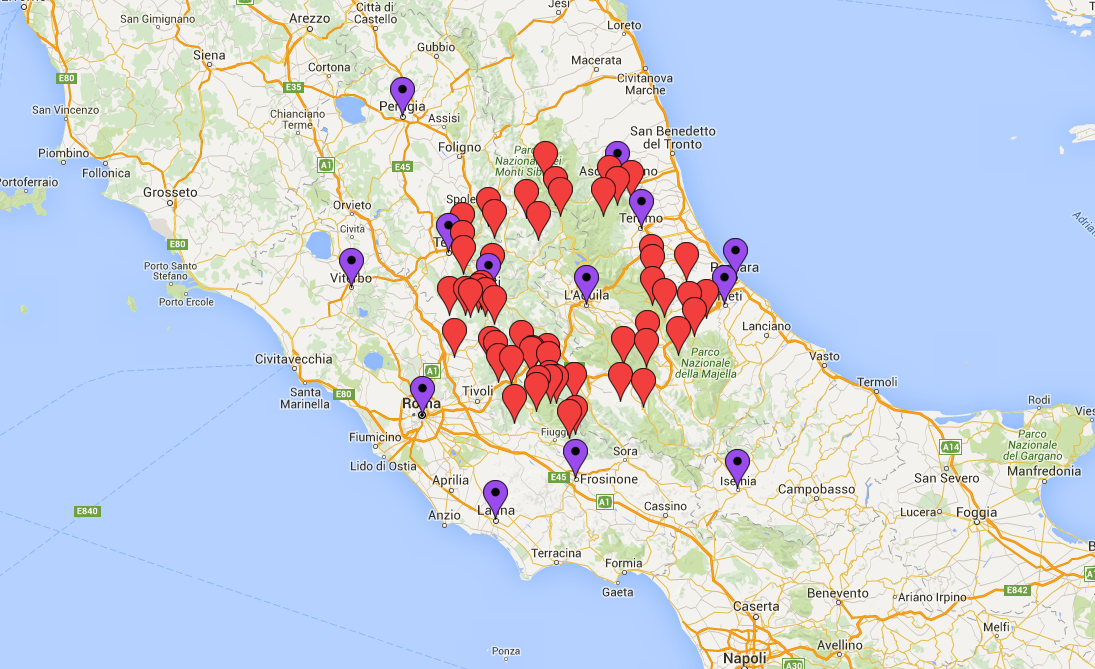
\includegraphics[keepaspectratio=true,height=200pt]{simulazione}

\end{frame}
\begin{frame}
	\frametitle{SeismoCloud: app per cellulari}
	
	\begin{itemize}
		\item Android, iOS
		\item Gratuita, presente nei canali ufficiali di distribuzione
		\item Contribuisce al rilevamento dei terremoti analizzando le vibrazioni (quando è poggiato su un tavolo)
		\item Riceve le notifiche di Early Warning
	\end{itemize}
	
\end{frame}
\begin{frame}
	\frametitle{SeismoCloud: il sismometro fisso}
	
	\begin{itemize}
		\item Schede principali: Intel Galileo, Raspberry PI + un accelerometro
		\item Sorgente libero e aperto (FOSS)
		\item Sistema operativo GNU/Linux
		\item Istruzioni sulla costruzione e funzionamento sul sito www.seismocloud.com
	\end{itemize}
	
	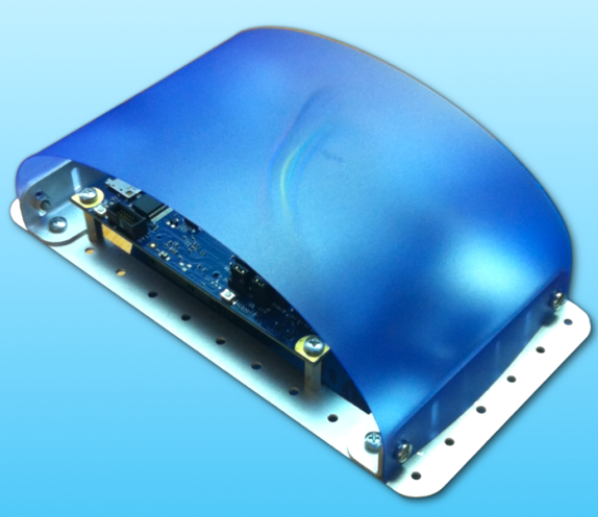
\includegraphics[keepaspectratio=true,width=100pt]{galileo}
	
\end{frame}
